% ---------------------------------------------------------------------------
% ---------------------------------------------------------------------------
% Modelo LaTex para preparação do documento final de Monografia TCC
% O modelo está em conformidade com ABNT NBR
% Faculdade do Piaui
% ---------------------------------------------------------------------------
% ---------------------------------------------------------------------------

\documentclass[
	% -- opções da classe memoir --
	12pt,					% tamanho da fonte
	openright,				% capítulos começam em pág ímpar (insere página vazia caso preciso)
	twoside,					% para impressão em verso e anverso. Oposto a oneside
	a4paper,					% tamanho do papel. 
	% -- opções da classe abntex2 --
	%chapter=TITLE,			% títulos de capítulos convertidos em letras maiúsculas
	%section=TITLE,			% títulos de seções convertidos em letras maiúsculas
	%subsection=TITLE,		% títulos de subseções convertidos em letras maiúsculas
	%subsubsection=TITLE,	% títulos de subsubseções convertidos em letras maiúsculas
	% -- opções do pacote babel --
	english,					% idioma adicional para hifenização
	%french,					% idioma adicional para hifenização
	%spanish,				% idioma adicional para hifenização
	brazil					% o último idioma é o principal do documento
	]{abntex2}

% ---------------------
% Pacotes OBRIGATÓRIOS
% ---------------------
\usepackage{lmodern}				% Usa a fonte Latin Modern			
\usepackage[T1]{fontenc}			% Selecao de codigos de fonte.
\usepackage[utf8]{inputenc}		% Codificacao do documento (conversão automática dos acentos)
\usepackage{lastpage}			% Usado pela Ficha catalográfica
\usepackage{indentfirst}			% Indenta o primeiro parágrafo de cada seção.
\usepackage{color}				% Controle das cores
\usepackage{graphicx,graphicx}	% Inclusão de gráficos
\usepackage{epsfig,subfig}		% Inclusão de figuras
\usepackage{microtype} 			% Melhorias de justificação
\graphicspath{{figs/}}
\usepackage[table,xcdraw]{xcolor}
% ---------------------
		
% ---------------------
% Pacotes ADICIONAIS
% ---------------------
\usepackage{pdfpages}


\usepackage{lipsum}						% Geração de dummy text
\usepackage{amsmath,amssymb,mathrsfs}	% Comandos matemáticos avançados 
\usepackage{setspace}  					% Para permitir espaçamento simples, 1 1/2 e duplo
\usepackage{verbatim}					% Para poder usar o ambiente "comment"
\usepackage{tabularx} 					% Para poder ter tabelas com colunas de largura auto-ajustável
\usepackage{afterpage} 					% Para executar um comando depois do fim da página corrente
\usepackage{url} 						% Para formatar URLs (endereços da Web)

%\usepackage[style=long,nonumberlist,toc,xindy,nomain]{glossaries}
				% para fazer glossario	
\usepackage{glossaries}	
\loadglsentries{extras/glossary}
\makeglossaries

%% para referenciar abreviaturas
\makeatletter
\def\namedlabel#1#2{\begingroup
	#2%
	\def\@currentlabel{#2}%
	\phantomsection\label{#1}\endgroup
}
% ---------------------

% ---------------------
% Pacotes de CITAÇÕES
% ---------------------
\usepackage[brazilian,hyperpageref]{backref}	% Paginas com as citações na bibl
\usepackage[alf]{abntex2cite}				% Citações padrão ABNT (alfa)
%\usepackage[num]{abntex2cite}				% Citações padrão ABNT (numericas)
% ---------------------

\usepackage{ulem}

\definecolor{mypurple}{rgb}{0.8,0.5,1}
\newcommand{\fulano}[1]{\textcolor{mypurple}{#1}}

\newcommand{\source}[1]{\caption*{Fonte: {#1}} }

% Configurações de CITAÇÕES para abntex2
% --- 
% CONFIGURAÇÕES DE PACOTES
% --- 

% ---
% Configurações do pacote backref
% Usado sem a opção hyperpageref de backref
\renewcommand{\backrefpagesname}{Citado na(s) página(s):~}
% Texto padrão antes do número das páginas
\renewcommand{\backref}{}
% Define os textos da citação
\renewcommand*{\backrefalt}[4]{
	\ifcase #1 %
		Nenhuma citação no texto.%
	\or
		Citado na página #2.%
	\else
		Citado #1 vezes nas páginas #2.%
	\fi}%
% ---

% Inclusão de dados para CAPA e FOLHA DE ROSTO (título, autor, orientador, etc.)
% ---
% Informações de dados para CAPA e FOLHA DE ROSTO
% ---
\titulo{Desenvolvimento de subsistemas para rotina de inspeção do Robô ELIR}
\autor{Carlos Pereira\\
	Cleber Couto Filho\\
	Davi Costa\\	
	Ícaro Queiroz\\}
\local{Salvador-BA}
\data{\today}
\orientador{Professor MSc. Marco Reis}
\coorientador{Professor(a) Titulação  Coorientador}
\instituicao{%
  Centro Universitário SENAI CIMATEC}
\tipotrabalho{Trabalho de Conclusão de Curso (TCC)}
% O preambulo deve conter o tipo do trabalho, o objetivo,
% o nome da instituição e a área de concentração
\preambulo{\textbf{Trabalho de Conclusão de Curso} apresentado ao Centro Universitário SENAI CIMATEC como requisito parcial para a obtenção do grau de Bacharel em Engenharia Elétrica.}
% ---

% Inclui Configurações de aparência do PDF Final
%  Configurações de aparência do PDF final
% NÃO ALTERAR!!!

% alterando o aspecto da cor azul
\definecolor{blue}{RGB}{41,5,195}

% informações do PDF
\makeatletter
\hypersetup{
     	%pagebackref=true,
		pdftitle={\@title}, 
		pdfauthor={\@author},
    		pdfsubject={\imprimirpreambulo},
	    pdfcreator={LaTeX with abnTeX2},
		pdfkeywords={abnt}{latex}{abntex}{abntex2}{trabalho acadêmico}, 
		colorlinks=true,       		% false: boxed links; true: colored links
    		linkcolor=blue,          	% color of internal links
    		citecolor=blue,        		% color of links to bibliography
    		filecolor=magenta,      		% color of file links
		urlcolor=blue,
		bookmarksdepth=4
} 
\makeatother
% --- 

% O tamanho da identação do parágrafo é dado por:
\setlength{\parindent}{1.3cm}

% Controle do espaçamento entre um parágrafo e outro:
\setlength{\parskip}{0.2cm}  % tente também \onelineskip

% ---------------------
% Compila o indice
% ---------------------
\makeindex
% ---------------------



%%%%%%%%%%%%%%%%%%%%%%%%%%%
%%  INICIO DO DOCUMENTO  %%
%%%%%%%%%%%%%%%%%%%%%%%%%%%
\begin{document}

% Retira espaço extra obsoleto entre as frases.
\frenchspacing

% ----------------------------------------------------------
% ELEMENTOS PRÉ-TEXTUAIS (Capa, Resumo, Abstract, etc.)
% ----------------------------------------------------------
\pretextual

% Capa
% ---
% Impressão da Capa
% ---
  \begin{capa}%
    \begin{figure}[h!]%
        \centering%
        
\includegraphics[scale=0.4]{figs/logo_senai.jpeg}%
      \end{figure}%
    \center
	\ABNTEXchapterfont\large{Centro Universitário SENAI CIMATEC\\Curso de Bacharelado em Engenharia Elétrica}
	%\vspace{1.5cm}

    \vfill
    \ABNTEXchapterfont\bfseries\LARGE\imprimirtitulo
    \vfill

	%\vfill
	\ABNTEXchapterfont\large\imprimirautor
	\vfill
%
    \large\imprimirlocal, \large\imprimirdata

    \vspace*{1cm}
  \end{capa}
% ---

% Folha de rosto (o * indica que haverá a ficha bibliográfica)
\imprimirfolhaderosto*

% Lista de ilustrações
\pdfbookmark[0]{\listfigurename}{lof}
\listoffigures*


% ----------------------------------------------------------
% ELEMENTOS TEXTUAIS (Capítulos)
% ----------------------------------------------------------
\textual
% Elementos textuais com numeração arábica
\pagenumbering{arabic}
% Reinicia a contagem do número de páginas
\setcounter{page}{1}

% Inclui cada capitulo da Dissertação
% ----------------------------------------------------------
% Introdução 
% Capítulo sem numeração, mas presente no Sumário
% ----------------------------------------------------------

\chapter*[Introdução]{Introdução}
\addcontentsline{toc}{chapter}{Introdução}

Este documento segue as normas estabelecidas pela~\citeonline[3.1-3.2]{NBR6028:2003}. \lipsum[30-34]

\section*{Motivação}\label{sec:motivacao}
\addcontentsline{toc}{section}{Motivação}

\lipsum[35]

\section*{Objetivos}\label{sec:objetivos}
\addcontentsline{toc}{section}{Objetivos}

Como objetivo geral este trabalho propõe...

Para isso, objetivos específicos foram assim definidos:

\begin{itemize}
\item especificar objetivos específicos
\item listar objetivos específicos
\end{itemize}

\section*{Organização do documento}\label{sec:objetivos}
\addcontentsline{toc}{section}{Organização do documento}

Parte I, Parte II, Parte III... \lipsum[32]


\chapter{Desenvolvimento}\label{cap:CnptDsng}

\section{Escolha da frequência}\label{sec:esc_freq}
A frequência foi escolhida com base no regulamento da Anatel. O mesmo estabelece que equipamentos de radiocomunicação com faixas restritas de: 902-907,5; 915-928; 2400-2483,5; 5725-5850 MHz, assim para os cálculos iniciais foi escolhida uma frequência de 920MHz.

\section{Estudo do Obstáculo}\label{sec:est_obs}
O primeiro passado adotado foi a análise dos pontos, verificando se entre os dois existia algum obstáculo. Essa informação pode ser extraída dos mapas que foram fornecidos em anexo, como mostra a figura \ref{fig:obs_cam}.
\begin{figure}[h]
	\centering
	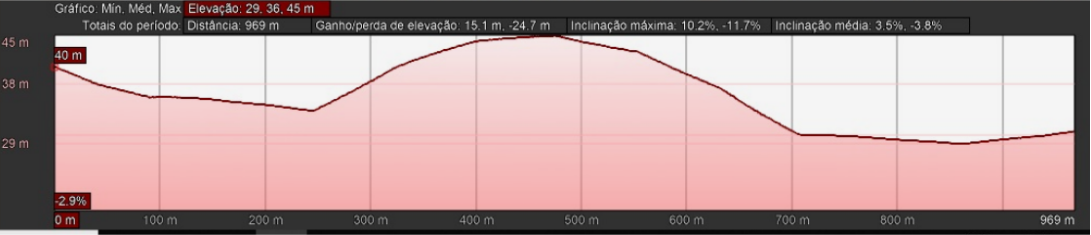
\includegraphics[width=1\textwidth]{obs_cam.png}
	\caption{Gráfico de obstáculo}
	\label{fig:obs_cam}
	%\source{Fornecido junto com os pontos}
\end{figure} 

Por meio da análise do gráfico, fica evidenciado que entre os dois pontos existe um grande obstáculo arredondado, assim sendo necessário calcular o seu raio de curvatura e a partir disso ver o quanto ele irá interferir na transmissão.
É feita uma aproximação do topo do obstáculo, utilizando uma curvatura parabólica como mostrado na figura 4 \ref{fig:obs_raio}.
\begin{figure}[h]
	\centering
	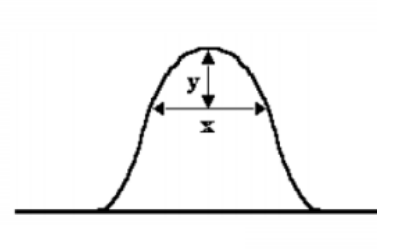
\includegraphics[width=.4\textwidth]{obs_raio.png}
	\label{fig:obs_raio}
	\caption{Curvatura parabólica utilizada para aproximação}
	%\source{Própria}
\end{figure} 

O raio $r$ da parábola será calculado o $\alpha$ que possibilita encontrar quantos decibéis de interferência o obstáculo irá causar. O cálculo do raio $r$ é feito utilizando a seguinte formula:
\begin{equation}
r = \dfrac{x^2}{8y}*10^{-3}
\end{equation}

Onde $x$ representa a distância em metros entre os dois pontos de igual nível, sendo um em cada lado do pico considerado e $y$ representa a diferença de cota entre o pico do obstáculo e a curva de nível considerada para  medida $x$. Com os dados de $x = 325m$ e $y = 7m$, o valor encontrado foi de $r = 1,886$

\section{Atenuação do Obstáculo}
O cálculo do fator $\alpha$ relaciona a frequência $f$, o raio de curvatura da parábola $r$, a distância entre o vértice do obstáculo ao ponto de transmissão $d_1 = 0.475$ e a distância entre o vértice do obstáculo ao ponto de recepção $d_2 = 0.492 $, ambas em \textit{Km}.
\begin{equation}
\alpha = 0,0818\dfrac{1}{\sqrt[6]{f}}\sqrt[3]{r}\sqrt{\dfrac{d_1+d_2}{d_1*d_2}}
\end{equation}

A atenuação é encontrada a partir de $\alpha$, que foi calculado com um valor de \textit{0.67} e a relação entre os fatores  $H_c$ e $r_f$ por meio do gráfico 5. Onde $H_c$ representa a diferença entre ponto máximo do obstáculo e o nivelamento das antenas, enquanto $r_f$  é chamado de raio de \textit{fresnel}, sendo calculado com as mesmas distâncias $d_1$ e $d_2$. A relação é encontrada como mostrado na figura 6.

\begin{figure}[h]
	\centering
	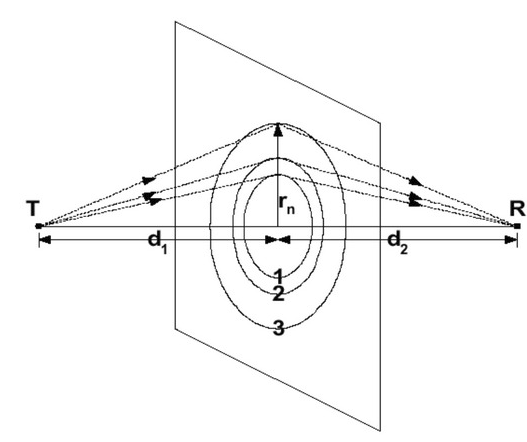
\includegraphics[width=.6\textwidth]{rf_img.png}
	\label{fig:rf_img}
	\caption{Modelo da zona de \textit{Fresnel}}
	%\source{Própria}
\end{figure}

O cálculo de $r_f$ se dá por:
\begin{equation}
r_f = \sqrt{\dfrac{n\lambda d_1 d_2}{d_1 + d_2}}
\end{equation}

\begin{figure}[h]
	\centering
	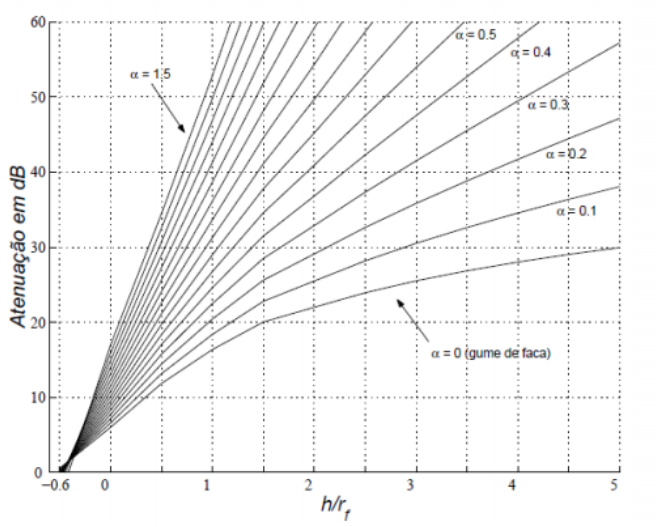
\includegraphics[width=.8\textwidth]{graf_ate.png}
	\label{fig:graf_ate}
	\caption{Gráfico de atenuação}
	%\source{Própria}
\end{figure} 

Onde o valor de $n$ foi fornecido como sendo igual a $1$ e com os valores mostrados na tabela e a análise do gráfico foi encontrado um valor de atenuação do obstáculo de $22,5dB$.

\begin{center}
	\begin{table}[]
		\begin{tabular}{|l|l|}
			\hline
			Rf    & 8,866 \\ \hline
			Hc    & 5     \\ \hline
			Hc/rf & 0,563 \\ \hline
		\end{tabular}
	\end{table}
\end{center}


\section{Atenuação no espaço livre}
O sinal também sofrerá atenuação ao ser transmitido no espaço livre, o cálculo da atenuação $L$ se dá por meio da fórmula de \textit{Fris}:
\begin{equation}
L = 32,45 +20(\log_{10}(d_1+d_2) + \log_{10}f)
\end{equation}

O valor encontrado foi de $L = 91,43dB$.

\section{Atenuação total}
A atenuação total é a soma da atenuação no espaço livre com a atenuação do obstáculo, assim :
\begin{equation}
L_{tot} = L + L_{obstaculo} = 91,43 + 22,5 = 113,9dB 
\end{equation}
\section{Escolha do tranmissor e da antena}
 A escolha dos módulos e da antena se deu baseado na frequência escolhida para os cálculos e na versatilidade de cada dispositivo. 
 
 O modelo das antenas foi o \textit{Yagi(AirMax Antenna 900Mhz)},devido a sua faixa de trabalho e alta potência.
 
 O modelo do transmissor foi o \textit{Ubiquiti Networks(Rocket M9)} pot ser recomendado para trabalhar em conjunto com o modelo de antena \textit{Yagi}. 
\section{Receptor}
O receptor é encontrado à partir das potências das antenas, do módulo tranmissor e das perdas durante a transmissão. Sua potência é calculada da seguinte forma:
%\begin{equation}
%	P_{receptor} = P_{antena_tx} + P_{antena_rx} + P_{transmissor} - L_{tot}
%\end{equation}

A mesma antena utilizada para transmissão é utilizada para recepção, os dados da sua potência estão disponíveis nos seu \textit{datasheet} onde $P_{antena_{tx}} = P_{antena_{rx}} = 19dBi$. A potência do transmissõr também está disponível no datasheet, onde $P_{transmissor} = 28dBm$. O valor encontrado para potência do receptor foi de $	P_{receptor} = -47.9dBi$

Com o valor de $-47.9dBi$, o módulo \textit{Ubiquiti Networks(Rocket M9)} também poderá ser utilizado para recepção, tornando o sistema mais simplificado já que ambos receptores e transmissores estarão utilizando antenas recomendadas no datasheet.

\chapter{Resultados}
Todos os valores utilizados e calculados estão registrados na figura a seguir:
\begin{figure}[h]
	\centering
	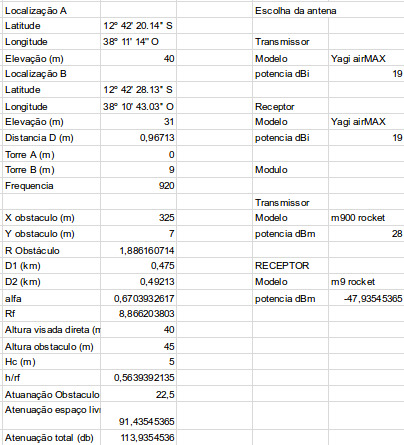
\includegraphics[width=1\textwidth]{resultados.jpeg}
	\label{fig:result}
	\caption{Variáveis do projeto}
	%\source{Própria}
\end{figure} 




%\chapter{Conclusão e Trabalhos Futuros}\label{cap:conclusao}

\lipsum[82-84]

\section{Trabalhos Futuros}

\lipsum[85] 

% ----------------------------------------------------------
% ELEMENTOS PÓS-TEXTUAIS (Referências, Glossário, Apêndices)
% ----------------------------------------------------------
\postextual

\begin{center}
	\Large \textbf{Referências}
\end{center}
	
	[1] TUDE, Eduardo. Enlace rádio digital ponto a ponto. 2004.

% Referências bibliográficas
%\bibliography{bibliografia}

%\printglossaries




% Índice remissivo (Consultar manual)
%\phantompart
%\printindex



\end{document}
